Material and Methods (Unsicher wie ich das aufbauen soll)

Netzwerk Architektur
Dataloading
Was ist Input
Wie werden Trainingsdaten erzeugt
Auswertungsmetriken

- Hypothesen und wie wir diese Überprüfen:
- ... 

Data:
Beschreibung der Patientendaten (wie viele, wie verteilt)
Infos zu der Ethical...
Falls in der Discussion die Feldgröße von Relevanz ist dann Infos mit rein nehmen. Nähere Infos in Tabelle

\subsection{Network Architecture}

3D UNet architecture with a downsampling ratio of 8 and a maximum layer depth of 512 in the bottleneck connection and skip connections before each pooling layer. multiple input masks in the size of CT with a resolution od 1.1718 x 1.1718 x 3 mm\textsuperscript{3} resolution in coronal, sagital, and tanversal dimension respectively. shown in image \autoref{fig:network}

\begin{figure}
    \centering
    \includegraphics[width=0.9\textwidth]{UNET.pdf}
    \caption{Network architeture scheme. Size of the input masks are depicted by width (W), height (H) and depth (D). Input dimensionality is WxHxDx5 and output dimensionality is WxHxDx1.}
    \label{fig:network}
\end{figure}

\subsection{Dataloading}

Patch based training, warum
erklären, dass aufgrund der Natur von 3D-Daten und dem Limit des Grafikkarten speichers nur ein teil der daten geladen werden können. erklären, dass der speicherpaltz verbrauch zum vorherigen abspeichern aller patches zu groß ist und die patches somit on the fly extrahiert werden mussen. eingehen auf TorchIO und deren lösung mittels einer queue an der sich meine lösung orientiert. on the fly loading von den daten in den datenspeicher und dann nach und nach füttern des Netzwerks mit gemischten Patches von verschiedenen patienten. verweis auf \autoref{fig:dataloading}

\begin{figure}
    \centering
    \includegraphics[width=0.9\textwidth]{dataloading.pdf}
    \caption{Memory efficient queue based dataloading for 3D patch based training. data from different segments are depicted in differnt color shades.}
    \label{fig:dataloading}
\end{figure}

\subsection{Network Input \& Output}



\subsubsection{Network Input}

The input consists of 5 3D volumes (\autoref{fig:masks}) to combine different spatial, anatomical aswell a accelorator information into the training data. the masks are used to achieve a direct connection from accelerator that translates onto the patients anatomy

\setlength{\hangingindent}{1em}
\begin{hangingpar}
    \item \textbf{Beam Shape}: beam shape information in form of a volume indicating the trajectory of the beam and its specific shape for each segment. in the masks voxels which the trajecotry passes contain the beam area. this accounts for the outputfactor of the accelerator, meaning that for bigger fields the in-scatter in the central beam line is higher than for smaller fields. 
\end{hangingpar}
\begin{hangingpar}
    \item \textbf{Center Beam Line Distance}: The beam of a linear accelerator is best defined in the central beam line. therefore the distance from the central beam line is of importance for the dose deposition. the minimum distance of each voxel from the central beam line accounting voxel dimensionality is saved in this mask.
\end{hangingpar}
\begin{hangingpar}
    \item \textbf{Source Distance}: The square rule of distance for the tissue in which the photons interact and the radiation source is of crucial importance for the dose deposited in the affected tissue. the values in this mask reflect the distance from each voxel to the radiation source with accounting the voxel dimensionality. 
\end{hangingpar}
\begin{hangingpar}
    \item \textbf{CT}: Dose deposition and particle interaction in genereal are defined by their energy aswell as the electron density of the affected volume. as the energy of the radiated photons is constant, the impact of the electron density of the volume (in this case the patients anatomy) is accounted in this mask. It consits of the houndsfield units from a ct scan. with this mask dose deposition in denser tissues can be accounted for.
\end{hangingpar}
\begin{hangingpar}
    \item \textbf{Radiological Depth}: as a particle passes trough the affected volume it loses its energy on its path. therefore the depth, which a particle has already passedd inside a tissue is very important for the dose deposition effects that take place. because particles lose their energy faster in dense materials, this affect is accounted for using the radiological depth. it accounts for the distance from the source as well as the electron density of the passed tissue. A depth in a dense material results in a higher radiological depth that the same depth in soft tissue.
\end{hangingpar}

To only clip the mask values to the actual patients anatomy, all values in each mask were set to zero where the CT mask had a HU value smaller than 874 (150 values above the HU value for air).

\begin{figure}
    \centering
    \includegraphics[width=\textwidth]{masks.pdf}
    \caption{From left to right: Beam Shape Mask, Center Beam Line Distance Mask, Source Distance Mask, CT Mask, Radiological Depth, Target Dose Mask}
    \label{fig:masks}
\end{figure}

\subsubsection{Network Output}

The output yielded by the network is the single volume of the predicted dose for the given input. It has the same dimensionality for wudthm height and depth aswell as voxel dimensions as the input masks. shown in \autoref{fig:masks}

\subsection{Training Data Generation}

The patient anatomy and accelerator information of each segment was extracted from the radio treatment plan. The required masks were created from this information using in-house python scripts. The target dose mask was simulated using the dosxyznrc software tool from the EGSnrc software package (the code is publicly available at https://github.com/nrc-cnrc/EGSnrc). EGSnrc enabled us to  us to simulate each beam segment from each patient's treatment plan, with the accurate MR linac accelerator head model frrom previous work at our institution. Each segment was simulated using 10\textsuperscript{7} for time efficiency. 

hier noch beschreiben wie lange due daten generation braucht? wichtig? 

\subsection{Evaluation Metrics}

to directly asses the quality of the dose prediction, we used the gamma - passrate, which compares two dose distrbutioins on the same grid. in this analysis tool eaach voxel and its value on grid 1 is compared to the zugehörigen voxel from the second dose distribution. two margins are used that define in which margin the seconds dose voxel can vary to be accepted as valid. the two margins are a dose value margin aswell as a spatial margin. hier noch erklären was der spatial margin eigentlich aussagt

heri noch vllt formel und abbildung die auswertungsmetrik

\subsection{Hypotheses}

\begin{hangingpar}
    \item\textbf{These 1}: the general dose deposition process for a spcific tumor entity can be learned on data of a multitude of radio treatment plans on that the specific tumor site. We therefore train a network on prostate patient treatment plan data and anatomies and assess the quality of predicted dose distribution with the gamma passrate of each segment as well asa the entire plan. 
\end{hangingpar}

\begin{hangingpar}
    \item\textbf{These 2}: the in These 1 trained network performes poorly when translating into different tumor sites that were not included in the training data and therefore generalizes poorly. To test translational capabilities the network is tested against liver, breast, head \& neck and lymph node treatment plan data.
\end{hangingpar}

\begin{hangingpar}
    \item\textbf{These 3}: the includation of different tumor sites into the training data improves the the translational capabilites of the network to other tumor sites, while maintaining high accuracy on the included tumor sites and therefore improve the robustness of the network. we therefore train the same network from these 1 on prostate, liver, breast and head \& neck treatment plan data. the translational capabilities are then assed by testing with prostate, liver, breast, head \& neck and lymph node data. by doing this we asses if the network performance decreases on prostate data by including new tumor sites into the training data and we assess its performance on seen (prostate, liver, heaad \& neck, breast) aswell as unseen treatment plan data (lymph nodes).
\end{hangingpar}

\begin{hangingpar}
    \item\textbf{These 4}: The network is capable of learning the underlying physics of the dose depositiopn process. By creating phantom input data in the form of a water slap at various positions inside an air volume, we investigate if the network has learned the underlying physics of the dose deposition process.
\end{hangingpar}

\subsection{Patient Data}

patient data from our institution previously treated at the mr linac. all plans were created by a medical physicist in agreement with a oncologist
Welche Entitäten: Prostate only training: 45 prostate treatment plans with a total of 2342 Segments, 36/4/5 split für train / val / test split. with a mean fieldsize of 36.57 ± 17.9 cm\textsuperscript{2} for training / validation set and 34.57 ± 15.86 cm\textsuperscript{2} for the test set.
mixed model 15 prostate with 720 segments , 35.49 ± 18.01 and 34.57 ± 15.86 15 liver 819 Segments 24.09 ± 18.36 and 22.81 ± 14.47 15 mamma 656 Segments 40.72 ± 28.48 and 40.60 ± 37.98 14 head \& neck 929 segments in einem 8/2/5 split also in 32/8/20 train / validation / test ratio. aswell as 15 patient plans 659 segments for lymphnodes exclusively for testing with a mean fieldsize of 25.95 ± 25.59
as you can see in \autoref{tab:patients}

63.00 ± 50.47
68.89 ± 53.56

\begin{table}
\centering
    \scalebox{0.7}{
        \begin{tabular}{|lcccccc|}
        \hline
                                            & \textbf{Prostate-Only}           & \multicolumn{4}{c}{\textbf{Mixed-Entity}}                                   & \textbf{Testing} \\ \hline
                                            & \multicolumn{1}{c|}{}            & Liver       & Mamma       & Head \& Neck & \multicolumn{1}{c|}{Prostate}    & Lymphnodes       \\
            Number of Segments              & \multicolumn{1}{c|}{45}          & 15          & 15          & 15           & \multicolumn{1}{c|}{15}          & 15               \\
            Number of Segments              & \multicolumn{1}{c|}{2342}        & 819         & 656         & 929          & \multicolumn{1}{c|}{720}         & 659              \\
            Training / Validation / Testing & \multicolumn{1}{c|}{36/4/5}      & 8/5/2       & 8/2/5       & 8/5/2        & \multicolumn{1}{c|}{8/5/2}       & Only Testing     \\
            Fieldsize Training/Validation   & \multicolumn{1}{c|}{36.5 (17.9)} & 24.1 (18.4) & 40.7 (28.5) & 63.0 (50.5)  & \multicolumn{1}{c|}{35.5 (18.0)} & N/A              \\
            Fieldsize Testing               & \multicolumn{1}{c|}{34.5 (15.8)} & 22.8 (14.4) & 40.6 (38.0) & 68.9 (53.6)  & \multicolumn{1}{c|}{34.6 (15.9)} & 26.0 (25.6)      \\ \hline
        \end{tabular}
    }
    \caption{Patient data infortmation for Prostate-Only as well as Mixed-Entity trained model and testing data set. Fieldsizes are given as mean (standard deviation).}
    \label{tab:patients}
\end{table}



% \textbf{\emph{Patient Data}}

% We used the treatment information from 45 prostate, 10 breast, 10 lymph node, 10 head and neck and 10 liver patients who were previoulsy treated using the MRI-Linac Elekta Unity (Elekta, Stockholm, Sweden) in our institution. \textbf{List fieldsizes, and gantry angle distribution (maybe a fanfy plot with a circualr coordinate system, like a distribution over angles) respectively}. 
% To to improve transational capabilities of the network 

% List how many segments for which entity I used and then how i split them up into training, validation and test patients and their respective number of segments. to match CT image shape dose distribution were resized to match the 512x512x number of slices shape of the ct input array. (siehe workflow\_code/utils.py skripte). The original iso center of the plan was used weather it was centered in the volume or not. 

% Ground truth dose distributions were calculated EGSnrc using 10\textsuperscript{7} histories. (information über EGSnrc also software version und release %\cite{noauthor_nrc-cnrcegsnrc_2021}) Each segment was calculated using same number of monitor units which enabled me to scale the segment based on the segment weight when predicting an entire treatment plan. 

% \textbf{\emph{Network}}

% The U-Net expects a 3d input of size (batchsize, num\_masks, W, H, D) and samples this input over the encoding path down to extract important features on a lower level scale from size [W, H, D] down to [W/2, H/2, D/2]. The decoding is done using 3D transposed convolutions with a kernelsize and a stride of 2 respectively. A skip connecting was added to before pooling to pass on highler level of volume resolution to later parts of the U-Net. 
% Each block building block consits of a convolutional layer with zero padding, to maintain dimensionality, kernel size 3$x$3$x$3 and a stride of 1, a 3D batch normalization layer and a RelU layer. No dropout was used. 
% Modified version of (doi:10.1007/978$-$3$-$319$-$24574$-$4\_28)


% % \begin{figure}
% % 	\centering
% %     \includegraphics[width=\textwidth]{UNET.pdf}
% %     \caption{3D U-Net architecture}
% %     \label{fig: unet}
% % \end{figure}

% % \begin{figure}
% % 	\centering
% %     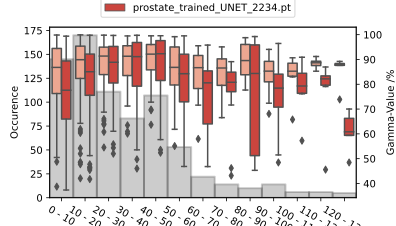
\includegraphics{test.pdf}
% %     \caption{Performance of the networks, trained on mixed and on prostate only patients anatomies and plan configurations. The underlying bar chart (left y axis) shows the occurneces of the fieldsizes listed on the x axis. The box plots (right y axis) shows the performance value of each discretized fieldsize range for both mixed and prostate only trained model. Outliers are depicted with a diamond shape}
% %     \label{fig: test}
% % \end{figure}

% % \begin{figure}
% % 	\centering
% %     \includegraphics{phantomP100T200_10x10_x.pdf}
% %     \caption{NONE}
% %     \label{fig: test}
% % \end{figure}
% % \begin{figure}
% % 	\centering
% %     \includegraphics{phantomP100T200_10x10_y.pdf}
% %     \caption{NONE}
% %     \label{fig: test}
% % \end{figure}

% % \begin{figure}
% % 	\centering
% %     \includegraphics{phantomP100T200_10x10_z.pdf}
% %     \caption{NONE}
% %     \label{fig: test}
% % \end{figure}

% % \begin{figure}
% % 	\centering
% %     \includegraphics{test_cases.pdf}
% %     \caption{NONE}
% %     \label{fig: test}
% % \end{figure}

% % \begin{figure}
% % 	\centering
% %     \includegraphics[width=\textwidth]{masks.pdf}
% %     \caption{Sample from a slice of training data. From left to right: beam shape, CT with Houndsfield Units, radiological depth, center beamline distance, source distance}
% %     \label{fig: test}
% % \end{figure}

% \textbf{\emph{Input Data}}

% The input of the network consists of 5 different masks containig spatial information about the given volume. (insert image with different masks and a little description of it) refer to deepdose paper by kontaxis %\cite{kontaxis_deepdose_2020}

% % \begin{figure}[H]
% %     \vspace{1cm}
% %     \minipage{0.32\textwidth}
% %         \includegraphics[width=4cm]{binary}
% %         \caption*{(a)}
% %     \endminipage\hfill
% %     \minipage{0.32\textwidth}
% %         \captionsetup{format=hang}
% %         \includegraphics[width=4cm]{ct.png}
% %         \caption*{(b)}
% %     \endminipage\hfill
% %     \minipage{0.32\textwidth}%
% %         \includegraphics[width=4cm]{radio.png}
% %         \caption*{(c)}
% %     \endminipage
% %     \vspace{1cm}
% %     \minipage{0.49\textwidth}
% %         \centering
% %         \includegraphics[width=4cm]{center}
% %         \caption*{(d)}
% %     \endminipage\hfill
% %     \minipage{0.49\textwidth}
% %         \centering
% %         \includegraphics[width=4cm]{source}
% %         \caption*{(e)}
% %     \endminipage\hfill
% %     \caption{Input masks for training}\label{fig: masks}
% % \end{figure}

% in the image above the the different input masks can bee seen. the masks are the binary beam shape (a), ct image with (electron density oder HU values, mal schauen was besser performed) (b) radiologial depth (c) center beamline distance (d) and source distance (d) 
% the binary beam shape input is most importance, due to the fact that this input mask is the only one providing the network with information about the beam position and orientation concerning shape and limits

% ct and readiological depth provide structural information about the parient anatomy. the radiological depth in particular helps the network to understand spatial dimensions when being given patches for training, becuase the information where a specific voxel is located inside the patients anatony would be lost when training with patches without the radiological depth. the algorithm for radiological depth calculation is implemented in python and based on  %\cite{siddon_fast_1985}

% all input masks are limited to the volume where the ct mask has a houndsfield unit value higher than 150, since this is the threshhold of our institunional dose esmiation software.

% The entire network and training algorithm is programmed in PyTorch. The dataloading was inspired by TorchIO, a libary for efficient dataloading for 3d medical imaging and especially patch based loading of 3d data. (torch io citen %\cite{perez-garcia_torchio_2021}) Due to the immense memory usage of (nummer an segmenten angeben) segments, not all segments could be loaded simutaneously into the memory. to archieve a randomised set of patches presented to the network at each training itteration, the dataloading is based on a subset of patient segments randomly selected from the entire training data pool. To further inprove dataloading time, a simutaneous loading of multiple segments at the same time using multi threading was implemented. 

% % \begin{figure}
% %     \centering
% %     \includegraphics[width=\textwidth]{dataloading.pdf}
% %     \caption{Dataloading scheme}\label{fig: dataloading}
% % \end{figure}

% % \begin{figure}
% %     \centering
% %     % This file was created with tikzplotlib v0.9.13.
\begin{tikzpicture}

\definecolor{color0}{rgb}{0.928267973856209,0.656699346405229,0.568464052287582}
\definecolor{color1}{rgb}{0.798039215686274,0.269607843137255,0.245098039215686}

\begin{axis}[
height=0.5\textwidth,
tick align=outside,
tick pos=left,
width=\textwidth,
x grid style={white!69.0196078431373!black},
xlabel={Fieldsize /\(\displaystyle cm^2\)},
xmin=-0.5, xmax=12.5,
xtick style={color=black},
xtick={0,1,2,3,4,5,6,7,8,9,10,11,12},
xticklabel style={rotate=330.0},
xticklabels={
  0 - 10,
  10 - 20,
  20 - 30,
  30 - 40,
  40 - 50,
  50 - 60,
  60 - 70,
  70 - 80,
  80 - 90,
  90 - 100,
  100 - 110,
  110 - 120,
  120 - 130
},
y grid style={white!69.0196078431373!black},
ylabel={Occurence},
ymin=0, ymax=178.5,
ytick style={color=black}
]
\draw[draw=black,fill=black,opacity=0.2,thick] (axis cs:-0.5,0) rectangle (axis cs:0.5,145);
\draw[draw=black,fill=black,opacity=0.2,thick] (axis cs:0.5,0) rectangle (axis cs:1.5,170);
\draw[draw=black,fill=black,opacity=0.2,thick] (axis cs:1.5,0) rectangle (axis cs:2.5,111);
\draw[draw=black,fill=black,opacity=0.2,thick] (axis cs:2.5,0) rectangle (axis cs:3.5,83);
\draw[draw=black,fill=black,opacity=0.2,thick] (axis cs:3.5,0) rectangle (axis cs:4.5,107);
\draw[draw=black,fill=black,opacity=0.2,thick] (axis cs:4.5,0) rectangle (axis cs:5.5,53);
\draw[draw=black,fill=black,opacity=0.2,thick] (axis cs:5.5,0) rectangle (axis cs:6.5,22);
\draw[draw=black,fill=black,opacity=0.2,thick] (axis cs:6.5,0) rectangle (axis cs:7.5,14);
\draw[draw=black,fill=black,opacity=0.2,thick] (axis cs:7.5,0) rectangle (axis cs:8.5,10);
\draw[draw=black,fill=black,opacity=0.2,thick] (axis cs:8.5,0) rectangle (axis cs:9.5,14);
\draw[draw=black,fill=black,opacity=0.2,thick] (axis cs:9.5,0) rectangle (axis cs:10.5,6);
\draw[draw=black,fill=black,opacity=0.2,thick] (axis cs:10.5,0) rectangle (axis cs:11.5,6);
\draw[draw=black,fill=black,opacity=0.2,thick] (axis cs:11.5,0) rectangle (axis cs:12.5,5);
\end{axis}

\begin{axis}[
axis y line=right,
height=0.5\textwidth,
legend cell align={left},
legend style={fill opacity=0.8, draw opacity=1, text opacity=1, at={(0.65,1.2)}, draw=white!80!black},
tick align=outside,
width=\textwidth,
x grid style={white!69.0196078431373!black},
xlabel={discrete},
xmin=-0.5, xmax=12.5,
xtick pos=left,
xtick style={color=black},
xtick={0,1,2,3,4,5,6,7,8,9,10,11,12},
xticklabels={10,20,30,40,50,60,70,80,90,100,110,120,130},
y grid style={white!69.0196078431373!black},
ylabel={Gamma-Value /\%},
ymin=34.248, ymax=103.042,
ytick pos=right,
ytick style={color=black},
yticklabel style={anchor=west}
]
\path [draw=white!31.3725490196078!black, fill=color0, semithick]
(axis cs:-0.396,76.265)
--(axis cs:-0.004,76.265)
--(axis cs:-0.004,94.445)
--(axis cs:-0.396,94.445)
--(axis cs:-0.396,76.265)
--cycle;
\path [draw=white!31.3725490196078!black, fill=color1, semithick]
(axis cs:0.004,65.97)
--(axis cs:0.396,65.97)
--(axis cs:0.396,89.41)
--(axis cs:0.004,89.41)
--(axis cs:0.004,65.97)
--cycle;
\path [draw=white!31.3725490196078!black, fill=color0, semithick]
(axis cs:0.604,82.335)
--(axis cs:0.996,82.335)
--(axis cs:0.996,95.38125)
--(axis cs:0.604,95.38125)
--(axis cs:0.604,82.335)
--cycle;
\path [draw=white!31.3725490196078!black, fill=color1, semithick]
(axis cs:1.004,75.5525)
--(axis cs:1.396,75.5525)
--(axis cs:1.396,92.17)
--(axis cs:1.004,92.17)
--(axis cs:1.004,75.5525)
--cycle;
\path [draw=white!31.3725490196078!black, fill=color0, semithick]
(axis cs:1.604,83.8925)
--(axis cs:1.996,83.8925)
--(axis cs:1.996,94.975)
--(axis cs:1.604,94.975)
--(axis cs:1.604,83.8925)
--cycle;
\path [draw=white!31.3725490196078!black, fill=color1, semithick]
(axis cs:2.004,80.505)
--(axis cs:2.396,80.505)
--(axis cs:2.396,95.26)
--(axis cs:2.004,95.26)
--(axis cs:2.004,80.505)
--cycle;
\path [draw=white!31.3725490196078!black, fill=color0, semithick]
(axis cs:2.604,83.51)
--(axis cs:2.996,83.51)
--(axis cs:2.996,95.535)
--(axis cs:2.604,95.535)
--(axis cs:2.604,83.51)
--cycle;
\path [draw=white!31.3725490196078!black, fill=color1, semithick]
(axis cs:3.004,79.235)
--(axis cs:3.396,79.235)
--(axis cs:3.396,96.85)
--(axis cs:3.004,96.85)
--(axis cs:3.004,79.235)
--cycle;
\path [draw=white!31.3725490196078!black, fill=color0, semithick]
(axis cs:3.604,85.8)
--(axis cs:3.996,85.8)
--(axis cs:3.996,96.04)
--(axis cs:3.604,96.04)
--(axis cs:3.604,85.8)
--cycle;
\path [draw=white!31.3725490196078!black, fill=color1, semithick]
(axis cs:4.004,81.525)
--(axis cs:4.396,81.525)
--(axis cs:4.396,97.605)
--(axis cs:4.004,97.605)
--(axis cs:4.004,81.525)
--cycle;
\path [draw=white!31.3725490196078!black, fill=color0, semithick]
(axis cs:4.604,79.7)
--(axis cs:4.996,79.7)
--(axis cs:4.996,95.04)
--(axis cs:4.604,95.04)
--(axis cs:4.604,79.7)
--cycle;
\path [draw=white!31.3725490196078!black, fill=color1, semithick]
(axis cs:5.004,72.92)
--(axis cs:5.396,72.92)
--(axis cs:5.396,92.12)
--(axis cs:5.004,92.12)
--(axis cs:5.004,72.92)
--cycle;
\path [draw=white!31.3725490196078!black, fill=color0, semithick]
(axis cs:5.604,78.2875)
--(axis cs:5.996,78.2875)
--(axis cs:5.996,91.61875)
--(axis cs:5.604,91.61875)
--(axis cs:5.604,78.2875)
--cycle;
\path [draw=white!31.3725490196078!black, fill=color1, semithick]
(axis cs:6.004,64.01125)
--(axis cs:6.396,64.01125)
--(axis cs:6.396,85.39)
--(axis cs:6.004,85.39)
--(axis cs:6.004,64.01125)
--cycle;
\path [draw=white!31.3725490196078!black, fill=color0, semithick]
(axis cs:6.604,79.55625)
--(axis cs:6.996,79.55625)
--(axis cs:6.996,90.24375)
--(axis cs:6.604,90.24375)
--(axis cs:6.604,79.55625)
--cycle;
\path [draw=white!31.3725490196078!black, fill=color1, semithick]
(axis cs:7.004,77.00375)
--(axis cs:7.396,77.00375)
--(axis cs:7.396,84.88)
--(axis cs:7.004,84.88)
--(axis cs:7.004,77.00375)
--cycle;
\path [draw=white!31.3725490196078!black, fill=color0, semithick]
(axis cs:7.604,83.82875)
--(axis cs:7.996,83.82875)
--(axis cs:7.996,96.05625)
--(axis cs:7.604,96.05625)
--(axis cs:7.604,83.82875)
--cycle;
\path [draw=white!31.3725490196078!black, fill=color1, semithick]
(axis cs:8.004,51.23375)
--(axis cs:8.396,51.23375)
--(axis cs:8.396,95.86875)
--(axis cs:8.004,95.86875)
--(axis cs:8.004,51.23375)
--cycle;
\path [draw=white!31.3725490196078!black, fill=color0, semithick]
(axis cs:8.604,80.98)
--(axis cs:8.996,80.98)
--(axis cs:8.996,89.2425)
--(axis cs:8.604,89.2425)
--(axis cs:8.604,80.98)
--cycle;
\path [draw=white!31.3725490196078!black, fill=color1, semithick]
(axis cs:9.004,70.77875)
--(axis cs:9.396,70.77875)
--(axis cs:9.396,84.07875)
--(axis cs:9.004,84.07875)
--(axis cs:9.004,70.77875)
--cycle;
\path [draw=white!31.3725490196078!black, fill=color0, semithick]
(axis cs:9.604,83.2625)
--(axis cs:9.996,83.2625)
--(axis cs:9.996,88.495)
--(axis cs:9.604,88.495)
--(axis cs:9.604,83.2625)
--cycle;
\path [draw=white!31.3725490196078!black, fill=color1, semithick]
(axis cs:10.004,76.36125)
--(axis cs:10.396,76.36125)
--(axis cs:10.396,84.43125)
--(axis cs:10.004,84.43125)
--(axis cs:10.004,76.36125)
--cycle;
\path [draw=white!31.3725490196078!black, fill=color0, semithick]
(axis cs:10.604,87.5375)
--(axis cs:10.996,87.5375)
--(axis cs:10.996,89.2875)
--(axis cs:10.604,89.2875)
--(axis cs:10.604,87.5375)
--cycle;
\path [draw=white!31.3725490196078!black, fill=color1, semithick]
(axis cs:11.004,79.6325)
--(axis cs:11.396,79.6325)
--(axis cs:11.396,83.3775)
--(axis cs:11.004,83.3775)
--(axis cs:11.004,79.6325)
--cycle;
\path [draw=white!31.3725490196078!black, fill=color0, semithick]
(axis cs:11.604,87.625)
--(axis cs:11.996,87.625)
--(axis cs:11.996,88.375)
--(axis cs:11.604,88.375)
--(axis cs:11.604,87.625)
--cycle;
\path [draw=white!31.3725490196078!black, fill=color1, semithick]
(axis cs:12.004,59.4)
--(axis cs:12.396,59.4)
--(axis cs:12.396,66.26)
--(axis cs:12.004,66.26)
--(axis cs:12.004,59.4)
--cycle;
\draw[draw=white!31.3725490196078!black,fill=color0,line width=0.3pt] (axis cs:0,0) rectangle (axis cs:0,0);
\addlegendimage{ybar,ybar legend,draw=white!31.3725490196078!black,fill=color0,line width=0.3pt}
\addlegendentry{mixed_trained_UNET_1183.pt}

\draw[draw=white!31.3725490196078!black,fill=color1,line width=0.3pt] (axis cs:0,0) rectangle (axis cs:0,0);
\addlegendimage{ybar,ybar legend,draw=white!31.3725490196078!black,fill=color1,line width=0.3pt}
\addlegendentry{prostate_trained_UNET_2234.pt}

\addplot [semithick, white!31.3725490196078!black, forget plot]
table {%
-0.2 76.265
-0.2 50.49
};
\addplot [semithick, white!31.3725490196078!black, forget plot]
table {%
-0.2 94.445
-0.2 99.855
};
\addplot [semithick, white!31.3725490196078!black, forget plot]
table {%
-0.298 50.49
-0.102 50.49
};
\addplot [semithick, white!31.3725490196078!black, forget plot]
table {%
-0.298 99.855
-0.102 99.855
};
\addplot [black, mark=diamond*, mark size=2.5, mark options={solid,fill=white!31.3725490196078!black}, only marks, forget plot]
table {%
-0.2 38.735
-0.2 48.775
};
\addplot [semithick, white!31.3725490196078!black, forget plot]
table {%
0.2 65.97
0.2 37.375
};
\addplot [semithick, white!31.3725490196078!black, forget plot]
table {%
0.2 89.41
0.2 99.395
};
\addplot [semithick, white!31.3725490196078!black, forget plot]
table {%
0.102 37.375
0.298 37.375
};
\addplot [semithick, white!31.3725490196078!black, forget plot]
table {%
0.102 99.395
0.298 99.395
};
\addplot [semithick, white!31.3725490196078!black, forget plot]
table {%
0.8 82.335
0.8 64.25
};
\addplot [semithick, white!31.3725490196078!black, forget plot]
table {%
0.8 95.38125
0.8 99.915
};
\addplot [semithick, white!31.3725490196078!black, forget plot]
table {%
0.702 64.25
0.898 64.25
};
\addplot [semithick, white!31.3725490196078!black, forget plot]
table {%
0.702 99.915
0.898 99.915
};
\addplot [black, mark=diamond*, mark size=2.5, mark options={solid,fill=white!31.3725490196078!black}, only marks, forget plot]
table {%
0.8 52.005
0.8 54.18
0.8 48.485
0.8 48.615
0.8 61.945
0.8 60.38
0.8 47.75
0.8 42.075
0.8 61.13
};
\addplot [semithick, white!31.3725490196078!black, forget plot]
table {%
1.2 75.5525
1.2 51.245
};
\addplot [semithick, white!31.3725490196078!black, forget plot]
table {%
1.2 92.17
1.2 99.79
};
\addplot [semithick, white!31.3725490196078!black, forget plot]
table {%
1.102 51.245
1.298 51.245
};
\addplot [semithick, white!31.3725490196078!black, forget plot]
table {%
1.102 99.79
1.298 99.79
};
\addplot [black, mark=diamond*, mark size=2.5, mark options={solid,fill=white!31.3725490196078!black}, only marks, forget plot]
table {%
1.2 47.74
1.2 46.625
1.2 41.765
1.2 46.52
1.2 46.05
1.2 45.445
};
\addplot [semithick, white!31.3725490196078!black, forget plot]
table {%
1.8 83.8925
1.8 68.77
};
\addplot [semithick, white!31.3725490196078!black, forget plot]
table {%
1.8 94.975
1.8 99.795
};
\addplot [semithick, white!31.3725490196078!black, forget plot]
table {%
1.702 68.77
1.898 68.77
};
\addplot [semithick, white!31.3725490196078!black, forget plot]
table {%
1.702 99.795
1.898 99.795
};
\addplot [black, mark=diamond*, mark size=2.5, mark options={solid,fill=white!31.3725490196078!black}, only marks, forget plot]
table {%
1.8 54.53
1.8 65.25
1.8 60.815
1.8 66.03
1.8 64.08
1.8 63.725
};
\addplot [semithick, white!31.3725490196078!black, forget plot]
table {%
2.2 80.505
2.2 61.05
};
\addplot [semithick, white!31.3725490196078!black, forget plot]
table {%
2.2 95.26
2.2 99.685
};
\addplot [semithick, white!31.3725490196078!black, forget plot]
table {%
2.102 61.05
2.298 61.05
};
\addplot [semithick, white!31.3725490196078!black, forget plot]
table {%
2.102 99.685
2.298 99.685
};
\addplot [black, mark=diamond*, mark size=2.5, mark options={solid,fill=white!31.3725490196078!black}, only marks, forget plot]
table {%
2.2 54.38
2.2 55.82
2.2 52.015
};
\addplot [semithick, white!31.3725490196078!black, forget plot]
table {%
2.8 83.51
2.8 71.23
};
\addplot [semithick, white!31.3725490196078!black, forget plot]
table {%
2.8 95.535
2.8 99.49
};
\addplot [semithick, white!31.3725490196078!black, forget plot]
table {%
2.702 71.23
2.898 71.23
};
\addplot [semithick, white!31.3725490196078!black, forget plot]
table {%
2.702 99.49
2.898 99.49
};
\addplot [black, mark=diamond*, mark size=2.5, mark options={solid,fill=white!31.3725490196078!black}, only marks, forget plot]
table {%
2.8 60.09
2.8 60.95
2.8 63.47
};
\addplot [semithick, white!31.3725490196078!black, forget plot]
table {%
3.2 79.235
3.2 53.56
};
\addplot [semithick, white!31.3725490196078!black, forget plot]
table {%
3.2 96.85
3.2 99.74
};
\addplot [semithick, white!31.3725490196078!black, forget plot]
table {%
3.102 53.56
3.298 53.56
};
\addplot [semithick, white!31.3725490196078!black, forget plot]
table {%
3.102 99.74
3.298 99.74
};
\addplot [black, mark=diamond*, mark size=2.5, mark options={solid,fill=white!31.3725490196078!black}, only marks, forget plot]
table {%
3.2 49.74
3.2 46.01
};
\addplot [semithick, white!31.3725490196078!black, forget plot]
table {%
3.8 85.8
3.8 72.8
};
\addplot [semithick, white!31.3725490196078!black, forget plot]
table {%
3.8 96.04
3.8 99.525
};
\addplot [semithick, white!31.3725490196078!black, forget plot]
table {%
3.702 72.8
3.898 72.8
};
\addplot [semithick, white!31.3725490196078!black, forget plot]
table {%
3.702 99.525
3.898 99.525
};
\addplot [black, mark=diamond*, mark size=2.5, mark options={solid,fill=white!31.3725490196078!black}, only marks, forget plot]
table {%
3.8 69.825
3.8 69.515
3.8 63.695
};
\addplot [semithick, white!31.3725490196078!black, forget plot]
table {%
4.2 81.525
4.2 57.685
};
\addplot [semithick, white!31.3725490196078!black, forget plot]
table {%
4.2 97.605
4.2 99.565
};
\addplot [semithick, white!31.3725490196078!black, forget plot]
table {%
4.102 57.685
4.298 57.685
};
\addplot [semithick, white!31.3725490196078!black, forget plot]
table {%
4.102 99.565
4.298 99.565
};
\addplot [black, mark=diamond*, mark size=2.5, mark options={solid,fill=white!31.3725490196078!black}, only marks, forget plot]
table {%
4.2 52.4
4.2 53.585
};
\addplot [semithick, white!31.3725490196078!black, forget plot]
table {%
4.8 79.7
4.8 61.845
};
\addplot [semithick, white!31.3725490196078!black, forget plot]
table {%
4.8 95.04
4.8 99.18
};
\addplot [semithick, white!31.3725490196078!black, forget plot]
table {%
4.702 61.845
4.898 61.845
};
\addplot [semithick, white!31.3725490196078!black, forget plot]
table {%
4.702 99.18
4.898 99.18
};
\addplot [black, mark=diamond*, mark size=2.5, mark options={solid,fill=white!31.3725490196078!black}, only marks, forget plot]
table {%
4.8 55.09
};
\addplot [semithick, white!31.3725490196078!black, forget plot]
table {%
5.2 72.92
5.2 46.86
};
\addplot [semithick, white!31.3725490196078!black, forget plot]
table {%
5.2 92.12
5.2 99.51
};
\addplot [semithick, white!31.3725490196078!black, forget plot]
table {%
5.102 46.86
5.298 46.86
};
\addplot [semithick, white!31.3725490196078!black, forget plot]
table {%
5.102 99.51
5.298 99.51
};
\addplot [semithick, white!31.3725490196078!black, forget plot]
table {%
5.8 78.2875
5.8 71.585
};
\addplot [semithick, white!31.3725490196078!black, forget plot]
table {%
5.8 91.61875
5.8 95.52
};
\addplot [semithick, white!31.3725490196078!black, forget plot]
table {%
5.702 71.585
5.898 71.585
};
\addplot [semithick, white!31.3725490196078!black, forget plot]
table {%
5.702 95.52
5.898 95.52
};
\addplot [black, mark=diamond*, mark size=2.5, mark options={solid,fill=white!31.3725490196078!black}, only marks, forget plot]
table {%
5.8 57.97
};
\addplot [semithick, white!31.3725490196078!black, forget plot]
table {%
6.2 64.01125
6.2 46.825
};
\addplot [semithick, white!31.3725490196078!black, forget plot]
table {%
6.2 85.39
6.2 95.79
};
\addplot [semithick, white!31.3725490196078!black, forget plot]
table {%
6.102 46.825
6.298 46.825
};
\addplot [semithick, white!31.3725490196078!black, forget plot]
table {%
6.102 95.79
6.298 95.79
};
\addplot [semithick, white!31.3725490196078!black, forget plot]
table {%
6.8 79.55625
6.8 66.545
};
\addplot [semithick, white!31.3725490196078!black, forget plot]
table {%
6.8 90.24375
6.8 95.07
};
\addplot [semithick, white!31.3725490196078!black, forget plot]
table {%
6.702 66.545
6.898 66.545
};
\addplot [semithick, white!31.3725490196078!black, forget plot]
table {%
6.702 95.07
6.898 95.07
};
\addplot [semithick, white!31.3725490196078!black, forget plot]
table {%
7.2 77.00375
7.2 71.635
};
\addplot [semithick, white!31.3725490196078!black, forget plot]
table {%
7.2 84.88
7.2 89.115
};
\addplot [semithick, white!31.3725490196078!black, forget plot]
table {%
7.102 71.635
7.298 71.635
};
\addplot [semithick, white!31.3725490196078!black, forget plot]
table {%
7.102 89.115
7.298 89.115
};
\addplot [black, mark=diamond*, mark size=2.5, mark options={solid,fill=white!31.3725490196078!black}, only marks, forget plot]
table {%
7.2 46.185
7.2 43.175
};
\addplot [semithick, white!31.3725490196078!black, forget plot]
table {%
7.8 83.82875
7.8 77.68
};
\addplot [semithick, white!31.3725490196078!black, forget plot]
table {%
7.8 96.05625
7.8 98.78
};
\addplot [semithick, white!31.3725490196078!black, forget plot]
table {%
7.702 77.68
7.898 77.68
};
\addplot [semithick, white!31.3725490196078!black, forget plot]
table {%
7.702 98.78
7.898 98.78
};
\addplot [semithick, white!31.3725490196078!black, forget plot]
table {%
8.2 51.23375
8.2 45.295
};
\addplot [semithick, white!31.3725490196078!black, forget plot]
table {%
8.2 95.86875
8.2 99.23
};
\addplot [semithick, white!31.3725490196078!black, forget plot]
table {%
8.102 45.295
8.298 45.295
};
\addplot [semithick, white!31.3725490196078!black, forget plot]
table {%
8.102 99.23
8.298 99.23
};
\addplot [semithick, white!31.3725490196078!black, forget plot]
table {%
8.8 80.98
8.8 72.365
};
\addplot [semithick, white!31.3725490196078!black, forget plot]
table {%
8.8 89.2425
8.8 94.065
};
\addplot [semithick, white!31.3725490196078!black, forget plot]
table {%
8.702 72.365
8.898 72.365
};
\addplot [semithick, white!31.3725490196078!black, forget plot]
table {%
8.702 94.065
8.898 94.065
};
\addplot [black, mark=diamond*, mark size=2.5, mark options={solid,fill=white!31.3725490196078!black}, only marks, forget plot]
table {%
8.8 68.075
};
\addplot [semithick, white!31.3725490196078!black, forget plot]
table {%
9.2 70.77875
9.2 51.515
};
\addplot [semithick, white!31.3725490196078!black, forget plot]
table {%
9.2 84.07875
9.2 96.45
};
\addplot [semithick, white!31.3725490196078!black, forget plot]
table {%
9.102 51.515
9.298 51.515
};
\addplot [semithick, white!31.3725490196078!black, forget plot]
table {%
9.102 96.45
9.298 96.45
};
\addplot [black, mark=diamond*, mark size=2.5, mark options={solid,fill=white!31.3725490196078!black}, only marks, forget plot]
table {%
9.2 48.475
};
\addplot [semithick, white!31.3725490196078!black, forget plot]
table {%
9.8 83.2625
9.8 82.975
};
\addplot [semithick, white!31.3725490196078!black, forget plot]
table {%
9.8 88.495
9.8 90.67
};
\addplot [semithick, white!31.3725490196078!black, forget plot]
table {%
9.702 82.975
9.898 82.975
};
\addplot [semithick, white!31.3725490196078!black, forget plot]
table {%
9.702 90.67
9.898 90.67
};
\addplot [black, mark=diamond*, mark size=2.5, mark options={solid,fill=white!31.3725490196078!black}, only marks, forget plot]
table {%
9.8 65.79
};
\addplot [semithick, white!31.3725490196078!black, forget plot]
table {%
10.2 76.36125
10.2 76.155
};
\addplot [semithick, white!31.3725490196078!black, forget plot]
table {%
10.2 84.43125
10.2 90.9
};
\addplot [semithick, white!31.3725490196078!black, forget plot]
table {%
10.102 76.155
10.298 76.155
};
\addplot [semithick, white!31.3725490196078!black, forget plot]
table {%
10.102 90.9
10.298 90.9
};
\addplot [black, mark=diamond*, mark size=2.5, mark options={solid,fill=white!31.3725490196078!black}, only marks, forget plot]
table {%
10.2 57.255
};
\addplot [semithick, white!31.3725490196078!black, forget plot]
table {%
10.8 87.5375
10.8 85.275
};
\addplot [semithick, white!31.3725490196078!black, forget plot]
table {%
10.8 89.2875
10.8 91.195
};
\addplot [semithick, white!31.3725490196078!black, forget plot]
table {%
10.702 85.275
10.898 85.275
};
\addplot [semithick, white!31.3725490196078!black, forget plot]
table {%
10.702 91.195
10.898 91.195
};
\addplot [semithick, white!31.3725490196078!black, forget plot]
table {%
11.2 79.6325
11.2 79.105
};
\addplot [semithick, white!31.3725490196078!black, forget plot]
table {%
11.2 83.3775
11.2 86.965
};
\addplot [semithick, white!31.3725490196078!black, forget plot]
table {%
11.102 79.105
11.298 79.105
};
\addplot [semithick, white!31.3725490196078!black, forget plot]
table {%
11.102 86.965
11.298 86.965
};
\addplot [black, mark=diamond*, mark size=2.5, mark options={solid,fill=white!31.3725490196078!black}, only marks, forget plot]
table {%
11.2 45.585
};
\addplot [semithick, white!31.3725490196078!black, forget plot]
table {%
11.8 87.625
11.8 87.625
};
\addplot [semithick, white!31.3725490196078!black, forget plot]
table {%
11.8 88.375
11.8 89.21
};
\addplot [semithick, white!31.3725490196078!black, forget plot]
table {%
11.702 87.625
11.898 87.625
};
\addplot [semithick, white!31.3725490196078!black, forget plot]
table {%
11.702 89.21
11.898 89.21
};
\addplot [black, mark=diamond*, mark size=2.5, mark options={solid,fill=white!31.3725490196078!black}, only marks, forget plot]
table {%
11.8 73.885
};
\addplot [semithick, white!31.3725490196078!black, forget plot]
table {%
12.2 59.4
12.2 59.4
};
\addplot [semithick, white!31.3725490196078!black, forget plot]
table {%
12.2 66.26
12.2 70.015
};
\addplot [semithick, white!31.3725490196078!black, forget plot]
table {%
12.102 59.4
12.298 59.4
};
\addplot [semithick, white!31.3725490196078!black, forget plot]
table {%
12.102 70.015
12.298 70.015
};
\addplot [black, mark=diamond*, mark size=2.5, mark options={solid,fill=white!31.3725490196078!black}, only marks, forget plot]
table {%
12.2 48.475
};
\addplot [semithick, white!31.3725490196078!black, forget plot]
table {%
-0.396 86.8
-0.004 86.8
};
\addplot [semithick, white!31.3725490196078!black, forget plot]
table {%
0.004 77.61
0.396 77.61
};
\addplot [semithick, white!31.3725490196078!black, forget plot]
table {%
0.604 89.91
0.996 89.91
};
\addplot [semithick, white!31.3725490196078!black, forget plot]
table {%
1.004 85.0475
1.396 85.0475
};
\addplot [semithick, white!31.3725490196078!black, forget plot]
table {%
1.604 91.365
1.996 91.365
};
\addplot [semithick, white!31.3725490196078!black, forget plot]
table {%
2.004 88.88
2.396 88.88
};
\addplot [semithick, white!31.3725490196078!black, forget plot]
table {%
2.604 91.305
2.996 91.305
};
\addplot [semithick, white!31.3725490196078!black, forget plot]
table {%
3.004 91.14
3.396 91.14
};
\addplot [semithick, white!31.3725490196078!black, forget plot]
table {%
3.604 92.145
3.996 92.145
};
\addplot [semithick, white!31.3725490196078!black, forget plot]
table {%
4.004 92.31
4.396 92.31
};
\addplot [semithick, white!31.3725490196078!black, forget plot]
table {%
4.604 86.81
4.996 86.81
};
\addplot [semithick, white!31.3725490196078!black, forget plot]
table {%
5.004 84.26
5.396 84.26
};
\addplot [semithick, white!31.3725490196078!black, forget plot]
table {%
5.604 86.7025
5.996 86.7025
};
\addplot [semithick, white!31.3725490196078!black, forget plot]
table {%
6.004 80.5825
6.396 80.5825
};
\addplot [semithick, white!31.3725490196078!black, forget plot]
table {%
6.604 86.56
6.996 86.56
};
\addplot [semithick, white!31.3725490196078!black, forget plot]
table {%
7.004 80.8025
7.396 80.8025
};
\addplot [semithick, white!31.3725490196078!black, forget plot]
table {%
7.604 89.5525
7.996 89.5525
};
\addplot [semithick, white!31.3725490196078!black, forget plot]
table {%
8.004 84.3575
8.396 84.3575
};
\addplot [semithick, white!31.3725490196078!black, forget plot]
table {%
8.604 85.295
8.996 85.295
};
\addplot [semithick, white!31.3725490196078!black, forget plot]
table {%
9.004 78.455
9.396 78.455
};
\addplot [semithick, white!31.3725490196078!black, forget plot]
table {%
9.604 85.275
9.996 85.275
};
\addplot [semithick, white!31.3725490196078!black, forget plot]
table {%
10.004 79.305
10.396 79.305
};
\addplot [semithick, white!31.3725490196078!black, forget plot]
table {%
10.604 88.6525
10.996 88.6525
};
\addplot [semithick, white!31.3725490196078!black, forget plot]
table {%
11.004 82.1725
11.396 82.1725
};
\addplot [semithick, white!31.3725490196078!black, forget plot]
table {%
11.604 87.82
11.996 87.82
};
\addplot [semithick, white!31.3725490196078!black, forget plot]
table {%
12.004 60.84
12.396 60.84
};
\end{axis}

\end{tikzpicture}

% %     \caption{Dataloading scheme}\label{fig:test}
% % \end{figure}

% (referenz auf bild was dataloading verdeutlicht) shows the schematic process of preloading a data queue from which random patches are taken for each batch presented the network for training. when the queue gets filled with patches a by the user specified number of segments gets randomly selected from the pool. then another by the user specified number of random patch positions per segment are extracted from the entire volume. then the entire queue gets shuffled and is then emptied during the training process. after the dataqueue is empty it is refilled with new patches from not previously used segments.
% after all segments have been used for patch extraction, the list of available segments is reset.


% \subsection{Training}

% The 3D-UNet was trained on a HPC cloud based solution using a 4 Nvidia GTX 2080 Ti with 11GB of VRAM. The batchsize for training was 128 and the patch size was 32 in all dimensions resulting in the input shape of (128, 5, 32, 32, 32). Since 4 graphics cards were used each card processed 32 patches of size (5, 32, 32, 32) simutaneously. The spatial resolution of a 32 x 32 x 32 patch was 37.4 x 37.4 x 96 mm\textsuperscript{3} with voxel dimensionality of 1.17 x 1.17 x 3 mm\textsuperscript{3}. 
% The loss function used was the root mean squared error and the ADAM optimizer with a starting learning rate of 10\textsuperscript{-4}, and the standard settings for beta1, beta2 and epsilon of 0.9, 0.999 and 10-8 respectively. Learning rate was reduced by a factor of 10 when no improvement in the validation loss could be observed. 
% A validation step was done after the training queue has been refilled resulting in a validation step after 12800 patches with 64 segments per queue and 200 patches per segment. The overall accuracy regarding the 3mm/3\% gamma values was assessed every 5 queue refillings. Training was stopped when no validation loss improvement could be observed for 30 epochs after learning rate reduction to 10\textsuperscript{-6}.

% Training supervision was done using Tensorboard in which training loss, validation loss and a the gamma pass rate could be viewed during training. 


% \subsection{Output analysis}

% To assess the overall performance of the network a gamma anlysis (cite gamma paper) was perfomed. The settings for individual segments and total plan are shown in Table. 

% Hier mal noch mit den anderen diskutieren, was man noch machen könnte. DVH? oder sonstige analysen der Dosis. z.B. diese Dice analyse die ich geplant hatte, wo man einen Threshold setzt und dann schauen wie sehr sich die prozente überschneiden.

% \subsection{Testing}

% The model tested on only prostate patients was tested against all other entities so assess the translational capabilities of a model only trained on one entity. The model trained on prostate, liver, breast and head and neck radio treatment data, was evaluated on all entities trained on aswell as on lypmh nodes to asses the translation to a tumor entity which was not present in the training data.